\documentclass[tikz,border=8pt]{standalone}
% Shared look for every TikZ diagram. Load with \input{../../tools/tikz-style.tex}
\usepackage[T1]{fontenc}
\usepackage{lmodern}
\renewcommand{\sfdefault}{lmr}  % diagrams use the same serif as the text
\usetikzlibrary{arrows.meta, positioning, shapes.geometric, calc, fit, backgrounds}
\definecolor{cblue}{HTML}{4C78A8}
\definecolor{corange}{HTML}{F58518}
\definecolor{cgreen}{HTML}{54A24B}
\definecolor{cred}{HTML}{E45756}
\definecolor{cpurple}{HTML}{B279A2}
\definecolor{cgrey}{HTML}{6B6B6B}
\tikzset{
  every picture/.style={font=\sffamily, line width=1.2pt},
  box/.style={draw=#1, fill=#1!12, rounded corners=4pt, align=center, inner sep=7pt, minimum height=1.1cm},
  box/.default=cgrey,
  arrow/.style={-{Stealth[length=3mm]}, draw=cgrey, line width=1.4pt},
  title/.style={font=\sffamily\bfseries\Large},
  note/.style={font=\sffamily\small, text=cgrey, align=center},
}
\AtBeginDocument{\hyphenpenalty=10000 \exhyphenpenalty=10000}

\begin{document}
% Section 7.2: one transformer encoder block (Vaswani et al. 2017, section 3.1). After each sub-layer:
% LayerNorm(x + Sublayer(x)), applied to every word vector separately.
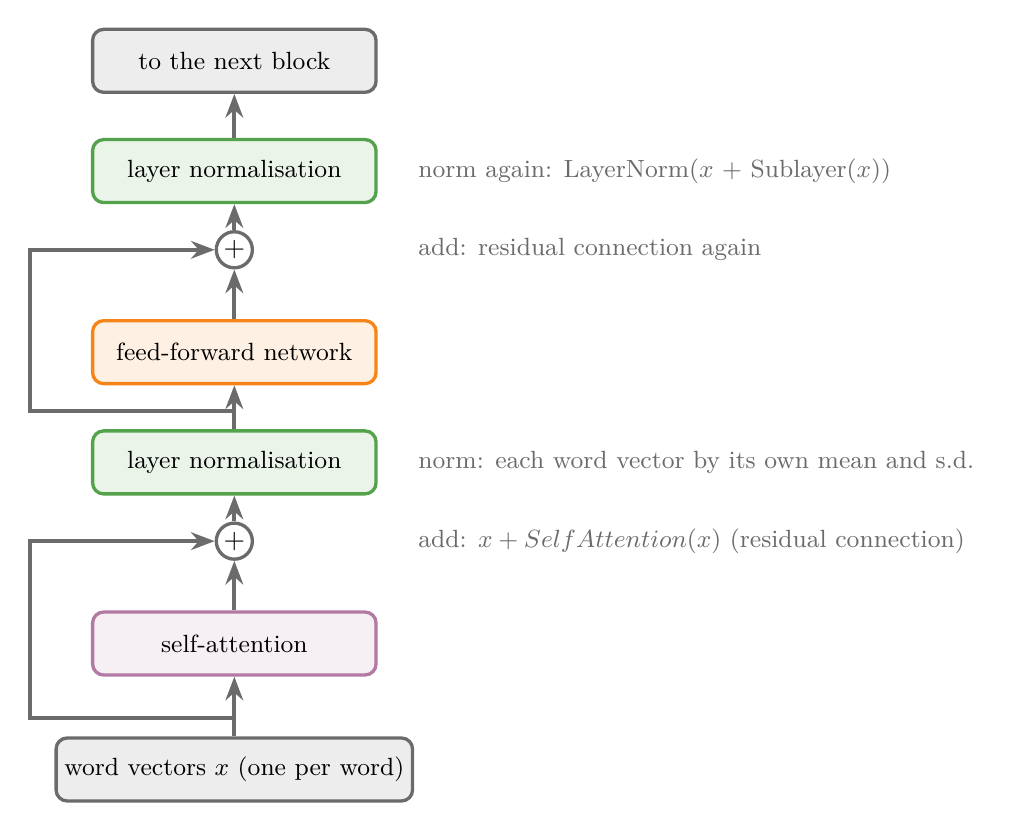
\begin{tikzpicture}[s/.style={box=#1, minimum width=3.6cm, minimum height=0.8cm, inner sep=3pt, font=\sffamily\small},
  plus/.style={circle, draw=cgrey, fill=white, inner sep=1pt, font=\sffamily\bfseries}]
  \node[s=cgrey] (x) at (0, 0) {word vectors $x$ (one per word)};
  \node[s=cpurple] (sa) at (0, 1.6) {self-attention};
  \node[plus] (p1) at (0, 2.9) {$+$};
  \node[s=cgreen] (ln1) at (0, 3.9) {layer normalisation};
  \node[s=corange] (ff) at (0, 5.3) {feed-forward network};
  \node[plus] (p2) at (0, 6.6) {$+$};
  \node[s=cgreen] (ln2) at (0, 7.6) {layer normalisation};
  \node[s=cgrey] (y) at (0, 9.0) {to the next block};
  \draw[arrow] (x) -- (sa); \draw[arrow] (sa) -- (p1); \draw[arrow] (p1) -- (ln1);
  \draw[arrow] (ln1) -- (ff); \draw[arrow] (ff) -- (p2); \draw[arrow] (p2) -- (ln2); \draw[arrow] (ln2) -- (y);
  \draw[arrow] (0, 0.65) -- (-2.6, 0.65) |- (p1.west);
  \draw[arrow] (0, 4.55) -- (-2.6, 4.55) |- (p2.west);
  \node[note, anchor=west] at (2.2, 2.9) {add: $x + \text{SelfAttention}(x)$ (residual connection)};
  \node[note, anchor=west] at (2.2, 3.9) {norm: each word vector by its own mean and s.d.};
  \node[note, anchor=west] at (2.2, 6.6) {add: residual connection again};
  \node[note, anchor=west] at (2.2, 7.6) {norm again: LayerNorm($x$ + Sublayer($x$))};
\end{tikzpicture}
\end{document}
